\documentclass[a4paper,titlepage]{article}
\usepackage[utf8]{inputenc}
\usepackage{fullpage}
\usepackage{indentfirst}
\usepackage[per-mode=symbol]{siunitx}
\usepackage{listings}
\usepackage{graphicx}
\usepackage{color}
\usepackage{amsmath}
\usepackage{array}
\usepackage[hidelinks]{hyperref}
\usepackage[format=plain,font=it]{caption}
\usepackage{subcaption}
\usepackage{standalone}
\usepackage[nottoc]{tocbibind}
\usepackage{cleveref}
\usepackage{titlesec}
\usepackage{booktabs}
\usepackage{csvsimple}
\usepackage[super]{nth}

% Custom commands
\newcommand\numberthis{\addtocounter{equation}{1}\tag{\theequation}}
\newcommand{\code}[1]{\texttt{#1}}
\newcolumntype{P}[1]{>{\centering\arraybackslash}p{#1}}

\titleformat*{\section}{\normalsize\bfseries}

%opening
\title{
	\textbf{ECSE 526 \\ Assignment 2}
	\\ \large Music Genre Classification
}
\author{Sean Stappas \\ 260639512}
\date{October \nth{19}, 2017}

\begin{document}
	\sloppy
	\maketitle
	\twocolumn
	
	\section{What assumptions about the data do we make when we model the data using a Gaussian distribution?}
	% Several key assumptions are stated.	
	% TODO: See 14.3, 20.2.3
	% Good reference: http://scikit-learn.org/stable/modules/neighbors.html
	
	Fundamentally, when we model the data using a Gaussian distribution, we assume that it has a Gaussian shape. This mainly implies the following:
	
	\begin{enumerate}
		\item The data has a mean.
		\item The data has a standard deviation.
		\item The data is symmetric around its mean.
	\end{enumerate}
	
	
	\section{When do you expect that a Gaussian will work well and when do you think it will not work well?}
	% Several situations are given, with elaborate discussion of the factors that make one classifier better than the other.
	
	A Gaussian classifier will work well when the data can be modeled with a Gaussian distribution, with the features listed in the previous question. This can be seen for instance in \autoref{fig:classical_gaussian}.
	
	\begin{figure}[!htb]
		\centering
		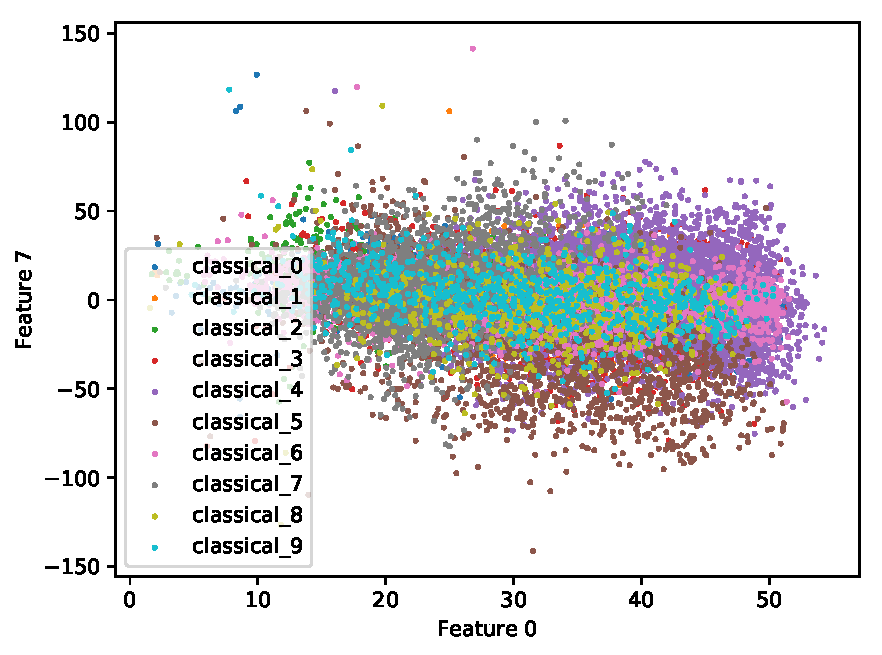
\includegraphics[width=\columnwidth]{plots/classical_gaussian.pdf}
		\caption
		{Projection of feature 0 vs. feature 7 for 10 songs from the ``classical'' genre. The distribution appears Gaussian.}
		\label{fig:classical_gaussian}
	\end{figure}
	
	% Examples of Gaussian working well: classical7
	
	A Gaussian classifier will not work in many situations. First, if the data itself cannot be modeled as Gaussian (using the assumptions in Question 1), then a Gaussian classifier will clearly not predict the correct values. For example, if the distribution is not symmetric, a Gaussian model will not work well. This can be seen in \autoref{fig:metal_non_symmetric}, where two features were plotted against each other for ten songs from the ``metal'' genre.
	
	% Non-symmetric examples: metal4, metal5
	
	\begin{figure}[!htb]
		\centering
		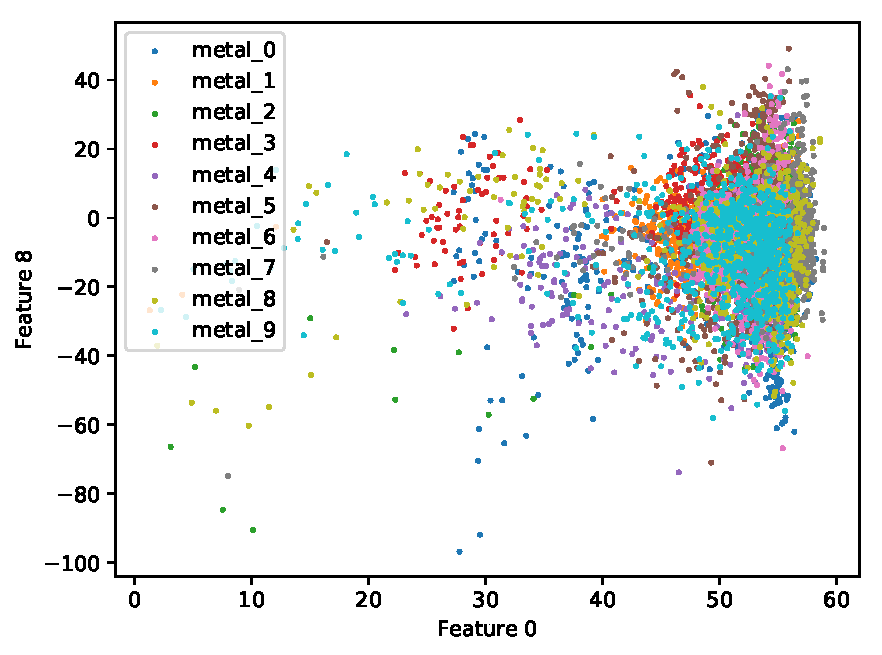
\includegraphics[width=\columnwidth]{plots/metal_non_symmetric.pdf}
		\caption
		{Projection of feature 0 vs. feature 8 for 10 songs from the ``metal'' genre. The distribution is not symmetric.}
		\label{fig:metal_non_symmetric}
	\end{figure}
	
	An example where a Gaussian model would not be appropriate is if, within a genre, there are multiple clusters of values. Here, multiple Gaussian distributions may be appropriate, but certainly not one. This can be seen in \autoref{fig:kids_cluster}, where two features were plotted against each other for ten songs from the ``kids'' genre.
	
	% Clustering examples: jazz19, jazz34, kids1, kids10, kids11, kids12, kids13, kids14, kids15, kids16, kids17
	
	\begin{figure}[!htb]
		\centering
		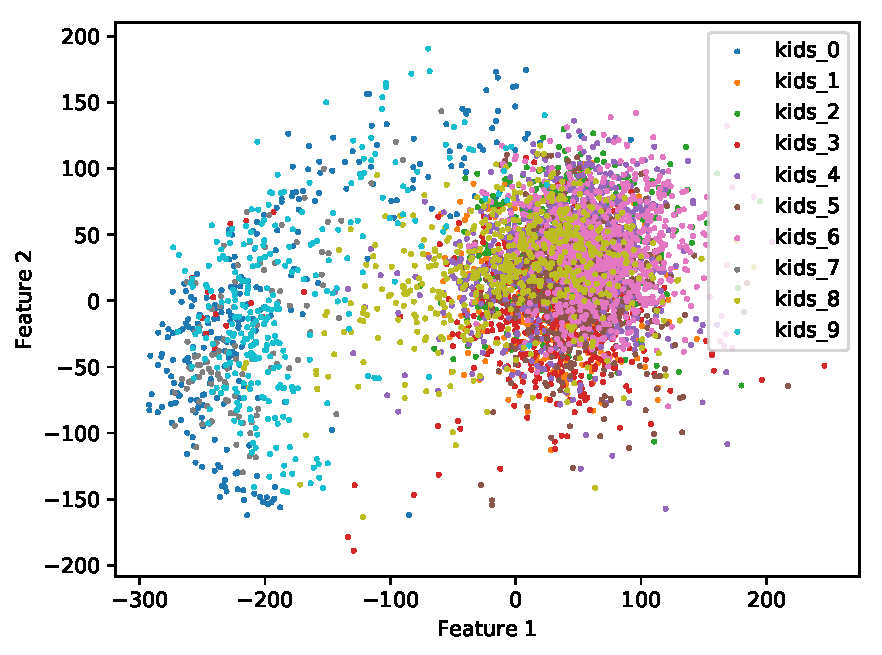
\includegraphics[width=\columnwidth]{plots/kids_cluster.pdf}
		\caption
		{Projection of feature 1 vs. feature 2 for 10 songs from the ``kids'' genre. Two separate clusters of values can be seen, on the left and the right.}
		\label{fig:kids_cluster}
	\end{figure}
	
	Secondly, if the feature vector distributions of two genres are very similar, then their corresponding Gaussian distributions will be very close, perhaps intersecting. In this situation, a Gaussian classifier can have a hard time differentiating between these two genres. This can be seen in \autoref{fig:latin_rnb_similarity}, where the ``latin'' and ``rnb'' genres have very similar distributions.
	
	\begin{figure}[!htb]
		\centering
		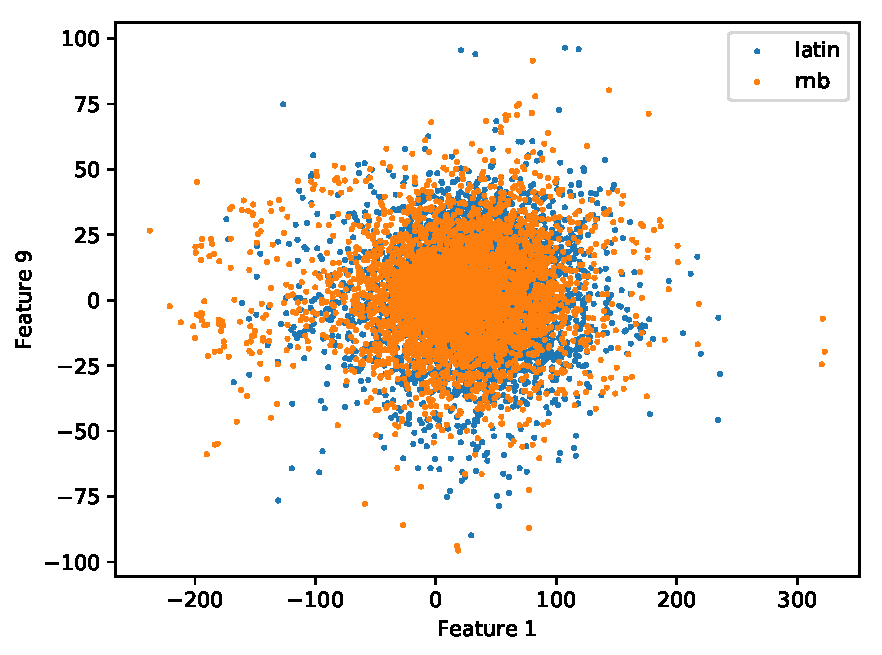
\includegraphics[width=\columnwidth]{plots/latin_rnb_similarity.pdf}
		\caption
		{Projection of feature 1 vs. feature 9 for 5 songs from the ``latin'' genre and 5 songs from the ``rnb'' genre. The distributions are very similar.}
		\label{fig:latin_rnb_similarity}
	\end{figure}
	
	Also, a Gaussian classifier will not work well for values that stray too far from the mean. In situations like this, kNN has the clear advantage. This can be seen in \autoref{fig:latin_extreme}, where two features were plotted against each other for ten songs from the ``latin'' genre.
	
	\begin{figure}[!htb]
		\centering
		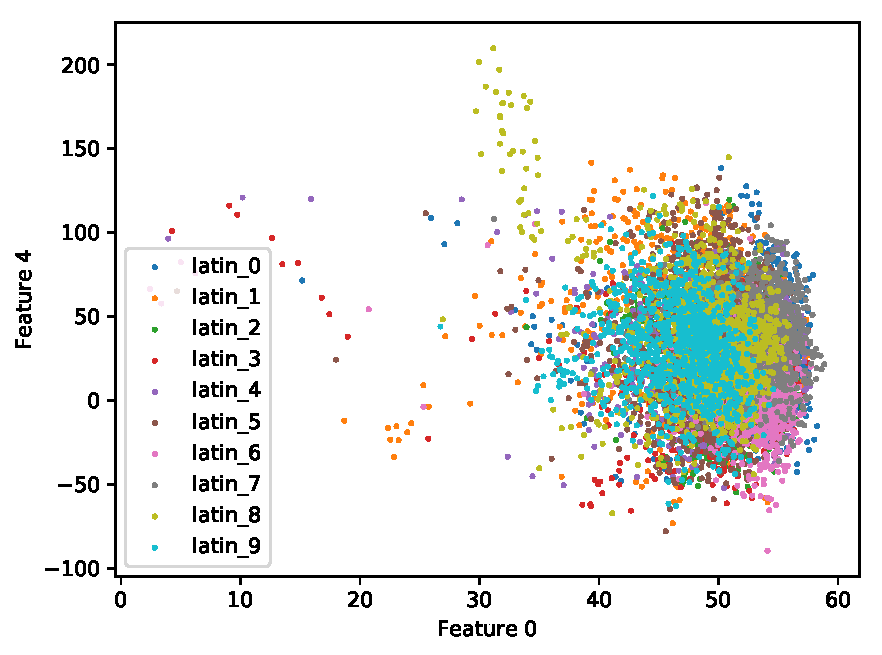
\includegraphics[width=\columnwidth]{plots/latin_extreme.pdf}
		\caption
		{Projection of feature 1 vs. feature 2 for 10 songs from the ``latin'' genre. There are many extreme values for which kNN would have an easier time classifying than Gaussian.}
		\label{fig:latin_extreme}
	\end{figure}
	
	
	\section{What values of $k$ work best for the kNN classifier?}
	% A value of k is stated, with a graph showing the results of different experiments.
	
	A common rule-of-thumb for the value of $k$ is that it should be equal to $\sqrt{N}$, where $N$ is the number of training samples. % TODO: Cite here
	
	After testing on various values of $k$, the best one was found to be % TODO: Show plot/table comparing values of k, choose best one
	
	\section{Based on your results from this assignment, which classifier (Gaussian or kNN) works best for the task of Music Genre Classification? Why?}
	% A classifier is stated as best, with elaboration on why, and with supporting evidence.
	
	The results of both classifiers can be seen in % TODO: accuracy for Gaussian and kNN
	
	\begin{table*}[!htb]
		\centering
		\caption{Confusion matrix for the Gaussian classifier. Each row represents the actual genre, and each column the predicted genre. The ordering of the column and row genres are the same.}
		\csvautobooktabular[respect all]{csv/confusion_gaussian.csv}
		\label{table:confusion_gaussian}
	\end{table*}

	\begin{table*}[!htb]
		\centering
		\caption{Confusion matrix for the kNN classifier, with $k = 1$. Each row represents the actual genre, and each column the predicted genre. The ordering of the column and row genres are the same.}
		\csvautobooktabular[respect all]{csv/confusion_knn_1.csv}
		\label{table:confusion_knn_1}
	\end{table*}
	
	Based on the above results, the kNN classifier works best for music classification. This can be attributed to the simple fact that the Gaussian classifier retains much less information than the kNN for each genre. While the Gaussian classifier only stores a 12x12 covariance matrix and 12x1 mean vector for each genre, the kNN classifier stores every training example and uses these examples to predict every genre. This additional information can allow the kNN classifier to classify new songs with much greater accuracy. 
	
	Also, kNN can take into account very complex distributions of feature vectors, whereas the Gaussian classifier will attempt to fit a Gaussian distribution to the data set, which may not be appropriate.
	
	% 
	
	%\renewcommand\refname{}
	%\bibliographystyle{unsrt}
	%\bibliography{readings}{}
	
\end{document}
